\documentclass[11pt]{article}
\usepackage[margin=1in]{geometry}
\usepackage{xcolor}
\usepackage{mdframed}
\usepackage{amsmath}
\usepackage{graphicx}
\usepackage{hyperref}
\usepackage{placeins}
\usepackage{booktabs}
\usepackage{float}

% copy cs555_hw_template.tex to cs555_hw_1_1.tex
\newcommand{\yourname}{Alex Shaffer, Istiaque Ahmed}
\newcommand{\yournetid}{aws9, miahmed2}
\newcommand{\hwnum}{2}
\newcommand{\probnum}{1}

\newenvironment{problem}[2][Problem]
    { \begin{mdframed}[backgroundcolor=gray!20] \textbf{#1 #2} \\}
    {  \end{mdframed}}

\newenvironment{solution}
    {\textit{Solution:}}
    {}

\begin{document}
\noindent
\noindent\rule{\linewidth}{2pt}
\large\textbf{\yourname} \hfill \textbf{CS 555: Homework \# \hwnum}   \\
Email: \yournetid@illinois.edu \hfill Spring 2026\\
\textbf{GitHub Repository:} \url{https://github.com/redhorn144/CS555}
\noindent\rule{\linewidth}{2pt}
\noindent
\begin{problem}{\probnum}
\textcolor{red}{optional: summarize the problem} % TODO
\end{problem}

\begin{solution}

(a)
For this part we have implemented a simple the point finite difference stencil to solve Burgers' equation. 
Plots of the solution for both Chebyshev and uniform nodes are shown in Figures \ref{fig:cheb1a} and \ref{fig:uni1a}, respectively.
For both of these N is taken to be 200, and the time step is taken to be smaller than the CFL constrint from part c.
Stapshots of the solution are taken at for $t = 0.1 k, \quad 0 \leq k \leq 20$.
In these particular cases we can see that the Chebyshev nodes do a better job at resolving the shock in the boundary layer.
This is because the Chebyshev nodes are clustered more closely together near the boundaries.
To be consistent with the paper we take $\nu = 1/100\pi$, but to be consistent with the homework handout we take $u^0 = \sin(\pi x)$ instead of $u^0 = -\sin(\pi x)$.

\begin{figure}[h!]
    \centering
    
\includegraphics[width=0.7\textwidth]{figures/1a_solution_chebyshev.png}
    \caption{Solutions to Burgers' equation with Chebyshev nodes.}
    \label{fig:cheb1a}
\end{figure}

\begin{figure}[h!]
    \centering
    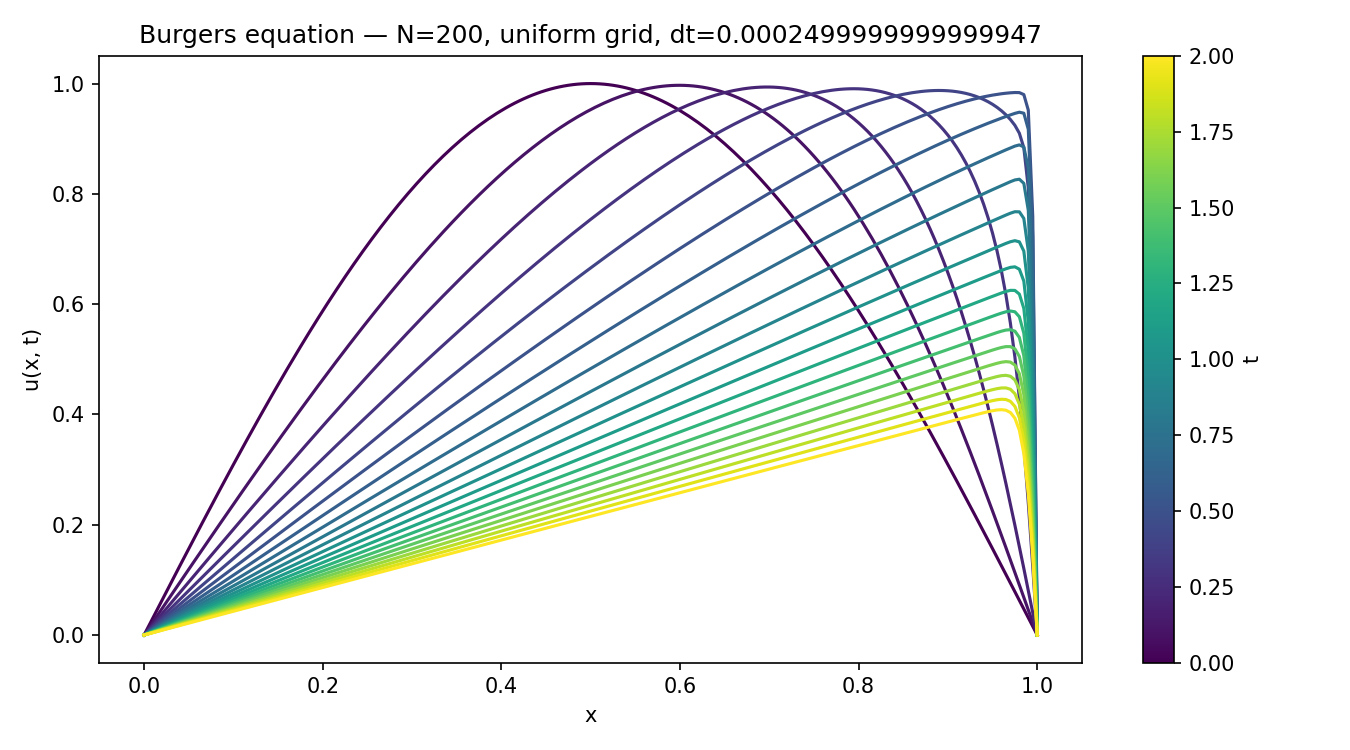
\includegraphics[width=0.7\textwidth]{figures/1a_solution_uniform.png}
    \caption{Solutions to Burgers' equation with uniform nodes.}
    \label{fig:uni1a}
\end{figure}

\FloatBarrier

(b)
Now we are asked to calculate the maximum value of the derivative of $u$ $s(t) = max_{x} |u_x(x,t)|$.
This is done with N = 200 again for both the uniform nodes and the Chebyshev nodes. 
The plot of $s(t)$ as well as $s^* = max_{t} s(t)$ is shown in Figures \ref{fig:cheb1b} and \ref{fig:uni1b} for the Chebyshev and uniform nodes, respectively.
The paper scales $t* = argmax s(t)$ by $\pi$. 
But without that scaling the analytical values of $s^*$ and $t^*$ are $s^* = 152.00516$ and $t^* = 0.51047$. 
The Chebyshev node case does notably better for determining $s^*$ and $t^*$.

\begin{figure}[h!]
    \centering
    
\includegraphics[width=0.7\textwidth]{figures/1b_smax_chebyshev.png}
    \caption{Your descriptive caption here.}
    \label{fig:cheb1b}
\end{figure}

\begin{figure}[h!]
    \centering
    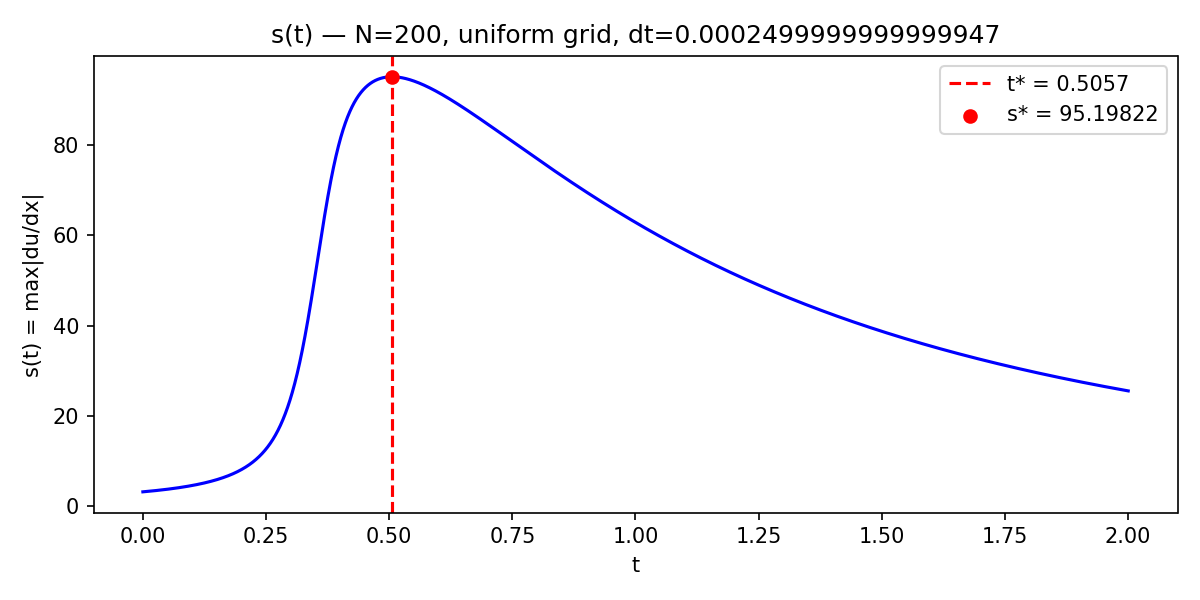
\includegraphics[width=0.7\textwidth]{figures/1b_smax_uniform.png}
    \caption{Your descriptive caption here.}
    \label{fig:uni1b}
\end{figure}

\FloatBarrier


(c)
Now, we push N with Chebyshev nodes up to 15000 and observe convergence of $s^*$ to the analytical value of $152.00516$.
We see, with that by N = 10000 we have a relative error of $4.552e-08$ which is on the order of the rounding error of the analytical value.
Because the table has $s^*$ out to 5 decimal places, as the analytical value is $152.00516$, we match by N = 10000.
This notably outperforms the uniform node case substantially.

\begin{table}[h!]
    \centering
    \begin{tabular}{|r|r|r|r|r|}
        \hline
        $N$ & $dt$ & nsteps & $s^*$ & rel\_err \\
        \hline
        25    & 3.864938e-03 & 518    & 72.28430  & 5.245e-01 \\
        50    & 1.960784e-03 & 1020   & 142.29624 & 6.387e-02 \\
        100   & 9.900990e-04 & 2020   & 151.39811 & 3.994e-03 \\
        200   & 4.975124e-04 & 4021   & 151.97705 & 1.849e-04 \\
        400   & 2.493766e-04 & 8021   & 152.00590 & 4.878e-06 \\
        800   & 1.248439e-04 & 16020  & 152.00583 & 4.419e-06 \\
        1500  & 6.662225e-05 & 30020  & 152.00538 & 1.481e-06 \\
        3000  & 3.332223e-05 & 60020  & 152.00522 & 3.941e-07 \\
        6000  & 1.666389e-05 & 120020 & 152.00517 & 1.073e-07 \\
        10000 & 9.999000e-06 & 200020 & 152.00516 & 4.552e-08 \\
        15000 & 6.666222e-06 & 300020 & 152.00516 & 2.601e-08 \\
        \hline
    \end{tabular}
    \caption{Convergence data for various $N$.}
    \label{tab:convergence}
\end{table}

\FloatBarrier

(d)
In this part we are asked to measure $s^*$ for the conservation form of Burgers' equation.
The plot of $s(t)$ for the conservation form is shown in Figure \ref{fig:cheb1b_cons}.
We are asked to compare this at the highest resolution to the convective form, and we see that they are very close to each other.
Infact they both predict $s^* = 152.00516$ to 5 decimal places, which is the same as the analytical value.
We see that the conservation form also converges to the analytical value as we increase N.
Part (e) elucidates the convergence behavior of both the convective and conservation forms for better comparison.


\begin{figure}[h!]
    \centering
    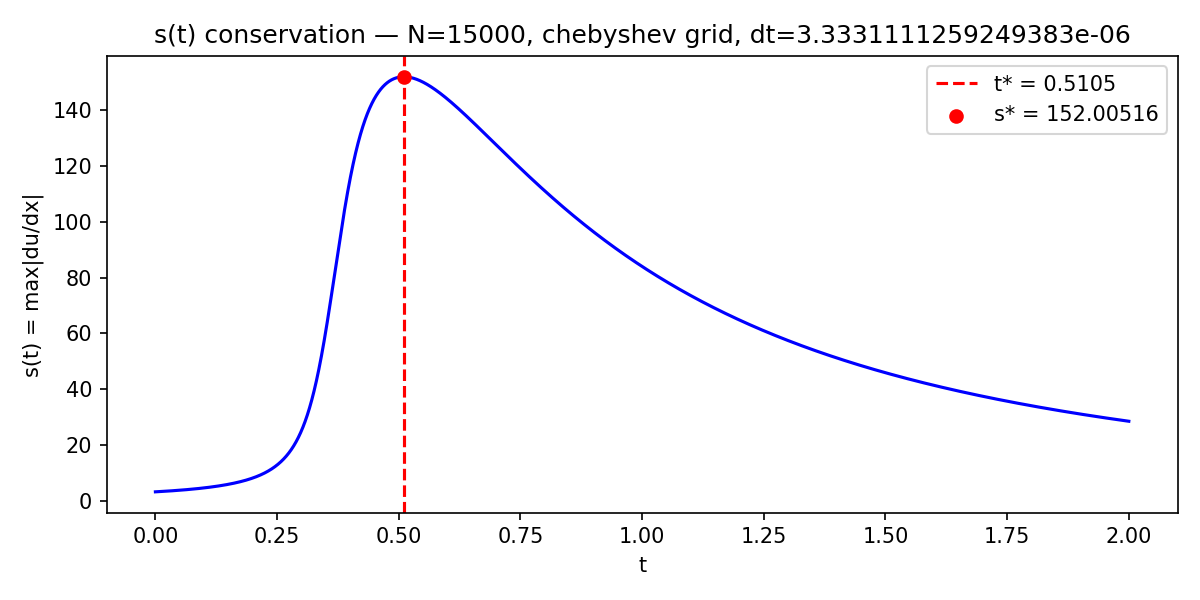
\includegraphics[width=0.7\textwidth]{figures/1b_cons_smax_chebyshev.png}
    \caption{Conservation of $s_{\max}$ using Chebyshev nodes.}
    \label{fig:cheb1b_cons}
\end{figure}

\FloatBarrier

(e)

The following tables document the convergence behavior for $N=2^k$ ($k=5, \dots, 11$) across four combinations of spatial discretization and nonlinear formulation. As instructed, the timestep $\Delta t = 0.1/N$, derived from the uniform grid CFL condition, is held constant across all cases to ensure a direct comparison without introducing variable time-stepping artifacts. The convergence ratio is defined as $\text{err}_{N/2}/\text{err}_{N}$.

\begin{table}[H]
\centering
\caption{Case i. Uniform spacing, convective form}
\begin{tabular}{@{}rrrrr@{}}
\toprule
$N$ & nsteps & $s^*$ & rel.err. & ratio \\
\midrule
  32 &   640 & 204.75163 & $3.47004 \times 10^{-1}$ & - \\
  64 &  1280 & 264.95618 & $7.43074 \times 10^{-1}$ & 0.467 \\
 128 &  2560 & 241.56922 & $5.89217 \times 10^{-1}$ & 1.261 \\
 256 &  5120 & 192.58263 & $2.66948 \times 10^{-1}$ & 2.207 \\
 512 & 10240 & 164.69320 & $8.34711 \times 10^{-2}$ & 3.198 \\
1024 & 20480 & 155.38910 & $2.22620 \times 10^{-2}$ & 3.749 \\
2048 & 40960 & 152.86551 & $5.66003 \times 10^{-3}$ & 3.933 \\
\bottomrule
\end{tabular}
\end{table}

\begin{table}[H]
\centering
\caption{Case ii. Chebyshev spacing, convective form}
\begin{tabular}{@{}rrrrr@{}}
\toprule
$N$ & nsteps & $s^*$ & rel.err. & ratio \\
\midrule
  32 &   640 & 167.45688 & $1.01653 \times 10^{-1}$ & - \\
  64 &  1280 & 153.42089 & $9.31369 \times 10^{-3}$ & 10.914 \\
 128 &  2560 & 152.11972 & $7.53643 \times 10^{-4}$ & 12.358 \\
 256 &  5120 & 152.01843 & $8.72962 \times 10^{-5}$ & 8.633 \\
 512 & 10240 & 152.00751 & $1.54404 \times 10^{-5}$ & 5.654 \\
1024 & 20480 & 152.00569 & $3.48080 \times 10^{-6}$ & 4.436 \\
2048 & 40960 & 152.00529 & $8.50164 \times 10^{-7}$ & 4.094 \\
\bottomrule
\end{tabular}
\end{table}

\begin{table}[H]
\centering
\caption{Case iii. Uniform spacing, conservation form}
\begin{tabular}{@{}rrrrr@{}}
\toprule
$N$ & nsteps & $s^*$ & rel.err. & ratio \\
\midrule
  32 &   640 &  65.52165 & $5.68951 \times 10^{-1}$ & - \\
  64 &  1280 & 102.90704 & $3.23003 \times 10^{-1}$ & 1.761 \\
 128 &  2560 & 140.71434 & $7.42792 \times 10^{-2}$ & 4.348 \\
 256 &  5120 & 157.73907 & $3.77218 \times 10^{-2}$ & 1.969 \\
 512 & 10240 & 156.53456 & $2.97977 \times 10^{-2}$ & 1.266 \\
1024 & 20480 & 153.55362 & $1.01869 \times 10^{-2}$ & 2.925 \\
2048 & 40960 & 152.42586 & $2.76767 \times 10^{-3}$ & 3.681 \\
\bottomrule
\end{tabular}
\end{table}

\begin{table}[H]
\centering
\caption{Case iv. Chebyshev spacing, conservation form}
\begin{tabular}{@{}rrrrr@{}}
\toprule
$N$ & nsteps & $s^*$ & rel.err. & ratio \\
\midrule
  32 &   640 & 159.19227 & $4.72820 \times 10^{-2}$ & - \\
  64 &  1280 & 153.81930 & $1.19348 \times 10^{-2}$ & 3.962 \\
 128 &  2560 & 152.15108 & $9.59988 \times 10^{-4}$ & 12.432 \\
 256 &  5120 & 152.01876 & $8.94915 \times 10^{-5}$ & 10.727 \\
 512 & 10240 & 152.00711 & $1.28268 \times 10^{-5}$ & 6.977 \\
1024 & 20480 & 152.00556 & $2.62221 \times 10^{-6}$ & 4.892 \\
2048 & 40960 & 152.00525 & $6.23135 \times 10^{-7}$ & 4.208 \\
\bottomrule
\end{tabular}
\end{table}

\subsubsection*{Discussion}
\begin{itemize}
    \item \textbf{Grid Spacing (Uniform vs. Chebyshev):} The uniform grid severely under-resolves the sharp internal layer at lower $N$ values, leading to significant numerical dispersion. This manifests as poor approximations of $s^*$ and erratic error convergence until $N \ge 1024$. In contrast, Chebyshev spacing naturally clusters grid points at the boundaries, placing high resolution precisely where the local gradients are maximized. Consequently, the Chebyshev cases reach an $\approx 10^{-5}$ relative error by just $N=256$, outperforming the uniform grid's finest resolution.
    \item \textbf{Convergence Ratio:} The theoretical error ratio for a second-order scheme when halving the spatial step size is $\approx 4$. For the Chebyshev grids (Cases ii and iv), the ratio rapidly stabilizes and approaches $\approx 4.1$ by the finest resolution, strictly confirming the scheme's second-order spatial accuracy. For uniform grids, the ratio behaves erratically before finally approaching the theoretical asymptotic value once the grid properly resolves the boundary layer at high $N$.
    \item \textbf{Formulation (Convective vs. Conservation):} At lower resolutions, the discrete truncation errors of the two forms lead to distinct failure modes; the convective form overestimates $s^*$ due to spurious oscillations, while the conservation form under-predicts it. However, once the grid is sufficiently refined (especially with Chebyshev spacing), both formulations converge to the analytical maximum $s^* \approx 152.005$ with nearly identical precision, robustly validating their formal equivalence.
\end{itemize}
\FloatBarrier

\end{solution} 

\end{document}